\chapter*{Preface}\label{preface}
% https://tex.stackexchange.com/questions/45672/adding-numberless-chapters-to-the-table-of-contents
\addcontentsline{toc}{chapter}{\protect\numberline{}Preface}
Modelica is a freely available, object-oriented language for modeling of
large, complex, and heterogeneous physical systems. From a user's point
of view, models are described by schematics, also called object
diagrams. Examples are shown in the next figure:

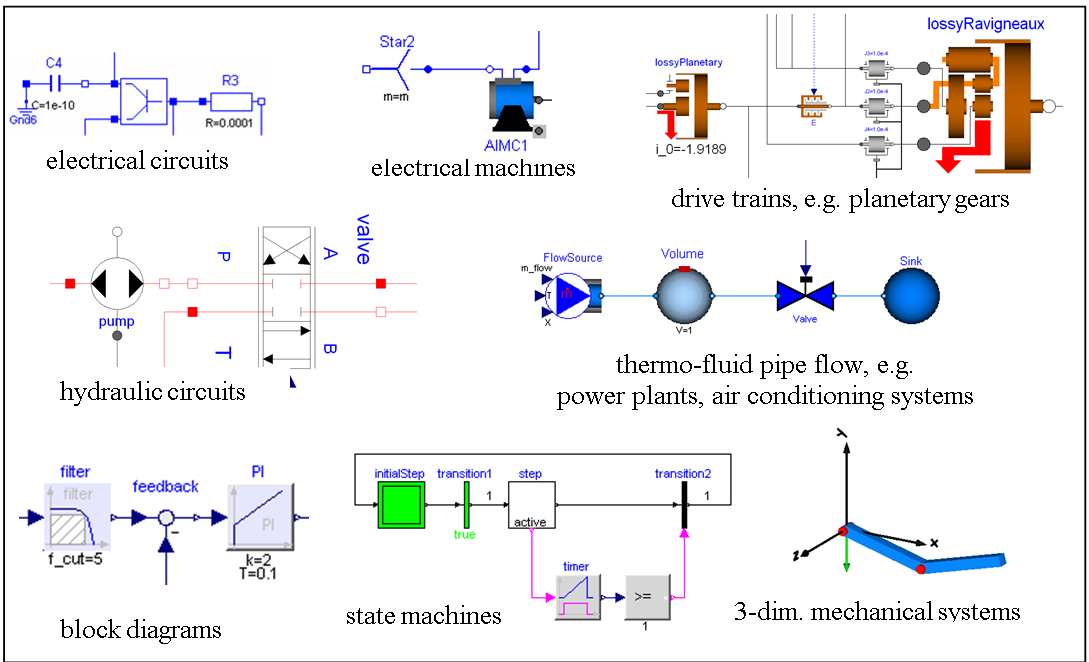
\includegraphics[width=5.92986in,height=3.59167in]{image2.png}

A schematic consists of connected components, like a resistor, or a
hydraulic cylinder. A component has \emph{connectors} (often also called
\emph{ports}) that describe the interaction possibilities, e.g., an
electrical pin, a mechanical flange, or an input signal. By drawing
connection lines between connectors a physical system or block diagram
model is constructed. Internally a component is defined by another
schematic, or on ``bottom'' level, by an equation-based description of
the model in Modelica syntax.

The Modelica language is a textual description to define all parts of a
model and to structure model components in libraries, called packages.
An appropriate Modelica simulation environment is needed to graphically
edit and browse a Modelica model (by interpreting the information
defining a Modelica model) and to perform model simulations and other
analysis. Information about such environments is available at
\href{https://www.modelica.org/tools}{www.modelica.org/tools}. Basically,
all Modelica language elements are mapped to differential, algebraic and
discrete equations. There are no language elements to describe directly
partial differential equations, although some types of discretized
partial differential equations can be reasonably defined, e.g., based on
the finite volume method and there are Modelica libraries to import
results of finite-element programs.

This document defines the details of the Modelica language. It is not
intended to learn the Modelica language with this text. There are better
alternatives, such as the Modelica books referenced at
\href{https://www.modelica.org/publications}{www.modelica.org/publications}.
This specification is used by computer scientist to implement a Modelica
translator and by modelers who want to understand the exact details of a
particular language element.

The Modelica language has been developed since 1996. This document
describes version 3.4 of the Modelica language. A complete summary is
available in \cref{modelica-3-4}.
